\chapter{Effects of alloying elements on the elastic properties of bcc Ti-X alloys}

\section{Introduction}

The present chapter is aimed at studying the effects of alloying elements on the mechanical properties of Ti-alloys as well as completing a database to calculate the elastic properties as a function of composition. This is accomplished by systematically studying the single crystal elastic stiffness constants (c$_{ij}$'s) and polycrystalline aggregate properties of bcc Ti-X (X = Mo, Nb, Ta, Sn, Zr) alloys. The elastic properties are calculated using first-principles calculations based on density functional theory (DFT). The composition dependence of the elastic properties of Ti-X alloys is explored through dilute solutions and special quasirandom structures (SQS) \cite{Jiang2004} for concentrated solutions using the methodologies outlined in chapter 2. The obtained elastic properties are then fit using the CALPHAD method and extrapolated to higher order Ti-alloys. 

\section{Modeling and Calculations}

\subsection{Calculation details}
In the present work, the Vienna ab-initio Simulation Package (VASP) \cite{Kresse1996} was employed to calculate the elastic properties of pure elements and Ti-containing binary systems in the bcc phase. The ion-electron interactions were described using the projector augmented wave (PAW) \cite{Kresse1999,Blochl1994} method. As discussed previously, the use of two X-C functionals were compared in this chapter and based on the results the generalized gradient approach depicted by Perdew, Burke, and Ernzerhof (PBE-GGA) was employed \cite{Perdew1996a}. For consistency, a 310 eV energy cutoff was adopted for all calculations, which is roughly 1.3 times higher than the default value. The energy convergence criterion of the electronic self-consistency was set as 10$^{-6}$ eV/atom, and the $\Gamma$-centered Monkhorst-Pack scheme was used for Brillouin zone sampling \cite{Kresse1996,Monkhorst1976a}. The k-points grid used for each calculation are listed in appendix C.

For the Ti-X binary systems, calculations for both dilute and SQS solutions were carried out. Three SQS cells with mole fractions of alloying element X atoms at 0.25, 0.5, and 0.75 were employed. Dilute solutions were calculated for each Ti-X binary alloy using different supercell sizes, i.e., Ti-Mo 4 dilute structures (Mo$_{0.98}$Ti$_{0.02}$ 54-atoms, Mo$_{0.94}$Ti$_{0.06}$ 16-atoms, Ti$_{0.88}$Mo$_{0.12}$ 8-atoms, Ti$_{0.94}$Mo$_{0.06}$ 16-atoms), Ti-Nb 4 dilute structures (Nb$_{0.98}$Ti$_{0.02}$ 54-atoms, Nb$_{0.94}$Ti$_{0.06}$ 16-atoms, Ti$_{0.88}$Nb$_{0.12}$ 8-atoms, Ti$_{0.98}$Nb$_{0.02}$ 54-atoms), Ti-Sn 1 dilute structure (Ti$_{0.94}$Sn$_{0.06}$ 16-atoms), Ti-Ta 5 dilute structures (Ta$_{0.98}$Ti$_{0.02}$ 54-atoms, Ta$_{0.94}$Ti$_{0.06}$ 16-atoms, Ti$_{0.88}$Ta$_{0.12}$ 8-atoms, Ti$_{0.94}$Ta$_{0.06}$ 16-atoms, Ti$_{0.98}$Ta$_{0.02}$ 54-atoms), Ti-Zr 2 dilute structures (Zr$_{0.94}$Ti$_{0.06}$ 16-atoms, Ti$_{0.98}$Zr$_{0.02}$ 54-atoms). The interaction parameters for the  elastic stiffness constants were then determined according to the methodology laid out in chapter 2.

\subsection{Modeling details}

The first-principles results were then used to model the elastic stiffness constants. The modeling was completed by calculating the difference between the first-principles calculations and a linear extrapolation between pure elements. The differences were then used to fit to the interaction parameters. Due to the limitations within the PARROT module, a Mathematica script was used to fit the interaction parameters. The Mathematica script is appended in appendix C. With the focus being Ti-rich alloys, the first-principles results with 70 at. \% Ti or higher were weighted heavier (x6, according to the authors' practices) than the other points for the fittings. The best fit was found by comparing the fittings obtained with one interaction parameter or with two interaction parameters. The moduli values were than calculated from the elastic stiffness constants according to the methodology in chapter 2.

\section{Results and discussion}

\subsection{Evaluation of calculation settings}

The X-C functionals of PW91 and PBE were tested on the Ti-Ta binary system. The results are plotted in Figure \ref{Ch5-figure:PBEvsPW91}, showing the $\overline{C}_{44}$ values differing by 10 GPa or less and the $\overline{C}_{11}$ and $\overline{C}_{12}$ values by less than 5 GPa for high Ta contents and by 26 GPa and 13 GPa with 25 at. \% Ta, respectively. Since overall the values vary by an error of less than 0.2 (calculated with Eq. \ref{eq: error}), and the PBE functional was developed as an improvement of the PW91 functional for metals, the PBE functional is chosen for the present work. 

Three magnitudes of strain are tested on the Ti-Mo binary system and plotted in Figure \ref{Ch5-figure:Strain}. The different strain magnitudes do not affect the results significantly. For example, the $\overline{C}_{11}$ values calculated using $\pm$0.01, $\pm$0.013, and $\pm$0.007 strains at Mo$_{0.94}$Ti$_{0.06}$ are 451 GPa, 450 GPa, and 450 GPa, respectively, varying within 1 GPa (< 0.01). The variances in the $\overline{C}_{12}$ and $\overline{C}_{44}$ results are similar. Overall, the variances in the $\overline{C}_{11}$ and $\overline{C}_{12}$ are less than 0.02 (Eq. \ref{eq: error}). The largest variance is in the Ti$_{0.50}$Mo$_{0.50}$ where the $\overline{C}_{44}$ values are 42 GPa, 42 GPa, and 65 GPa calculated with $\pm$0.01, $\pm$0.013, and $\pm$0.007 strains, respectively. Overall, the strain magnitude does not affect the calculated results significantly, and thus the $\pm$0.01 strain magnitude is used for all the calculations.

\subsection{Calculations of elastic coefficients in Ti-X binary systems}

The elastic stiffness coefficients and bulk moduli ($B$) are calculated for the pure elements in the bcc structure and reported in Table \ref{Ch5-table:pureeleelas}. The results in the present work are all obtained at 0 $^\circ$K. The results for Mo, Nb and Ta, which are stable in the bcc structure at low temperatures, are compared with experimental data at temperatures shown in Table \ref{Ch5-table:pureeleelas} \cite{Dickinson1967a,Bolef1961}. The error (Eq. \ref{eq: error}) between the present results and previous results for Mo, Nb and Ta are 0.0261, 0.075, and 0.0425, respectively \cite{Simmons1971b,Dickinson1967a,Bolef1961}. This discrepancy is due to the temperature difference between the experiments and calculations. The calculations are at 0 $^\circ$K while the experimental values were measured at higher temperatures. 

Ti and Zr are stable in the hcp structure at low temperatures, and Sn is stable in the body centered tetragonal and diamond structures at low temperatures. Due to the instability of Ti, Sn and Zr in the bcc structure at low temperatures, their elastic stiffness coefficients are compared to previous first-principles calculations at 0 $^\circ$K \cite{Shang2010b} that used the PW91 functional, and the errors/differences are 0.024, 0.528 and 0.051, respectively. The differences are related to the instability of the bcc structure, the different exchange correlation functionals and the different input parameters chosen. Due to the bcc instability, multiple relaxation schemes are compared in the present work to find the lowest energy structure retaining the bcc symmetry, making the results the most accurate representation of the bcc pure elements.  

Figure \ref{Ch5-figure:tixc11} to Figure \ref{Ch5-figure:tixc44} compare the calculated elastic stiffness coefficients, $\overline{C}_{11}$, $\overline{C}_{12}$, $\overline{C}_{44}$ (circles) with the currently modeled elastic stiffness coefficients (solid line) and linear combination from the pure elements for the Ti-Mo, Ti-Nb, Ti-Sn, Ti-Ta, and Ti-Zr systems. The model parameters are shown in Table \ref{Ch5-table:tixelasip}. The results calculated for the Ti-Mo, Ti-Nb, and Ti-Ta systems are compared with previous calculated results from Ikehata et al. \cite{Ikehata2004}, and the differences are due to the different input parameters and structures used at each composition. Ikehata et al. \cite{Ikehata2004} used the s orbital electrons as the valance electrons for Ti and used the B2 structure for their Ti$_{0.50}$X$_{0.50}$ compositions with Ti at the body centered site and X at the corner sites. For the Ti$_{0.25}$X$_{0.75}$ and Ti$_{0.75}$X$_{0.25}$ structures they used the DO$_{3}$ structure with space group $Fm\overline{3}m$, and not the bcc space group of $Im\overline{3}m$. The present work uses the p electrons as valance electrons for Ti based on updated recommendations by VASP and 16-atom SQS from Jiang et al. \cite{Jiang2004}. The SQS mimic the random substitution of elements with less error and represent the atomic structures of solution phases better than ordered structures. It can be seen that Mo, Nb, and Ta affect the elastic stiffness coefficients in a similar fashion. As shown in Figure \ref{Ch5-figure:tixc11}a, \ref{Ch5-figure:tixc11}b and \ref{Ch5-figure:tixc11}d the $\overline{C}_{11}$ increases in value from Ti to X (X = Mo, Nb, Ta). \ref{Ch5-figure:tixc44}a, \ref{Ch5-figure:tixc44}b and \ref{Ch5-figure:tixc44}d show that the $\overline{C}_{44}$ values first decrease and then increase with the addition of the alloying element X (X = Mo, Nb and Ta). The $\overline{C}_{12}$ values increase by the addition of Mo or Ta (Figure \ref{Ch5-figure:tixc12}a and Figure \ref{Ch5-figure:tixc12}d, respectively), and the $\overline{C}_{12}$ values first decrease and then increase by the addition of Nb (Figure \ref{Ch5-figure:tixc12}b). A similar trend is shown in the $\overline{C}_{11}$ and $\overline{C}_{12}$ data for the Ti-Sn system (Figure \ref{Ch5-figure:tixc11} and Figure \ref{Ch5-figure:tixc12}c). The $\overline{C}_{11}$ and $\overline{C}_{12}$ values first increase and then decrease from pure Ti to pure Sn. As seen in Figure \ref{Ch5-figure:tixc44}c, $\overline{C}_{44}$ first increases in value, then decreases, and then increases again from pure Ti to pure Sn. In the Ti-Zr system, the $\overline{C}_{11}$ and $\overline{C}_{44}$ values first increase and then decrease with increasing Zr concentration (Figure \ref{Ch5-figure:tixc11}e and Figure \ref{Ch5-figure:tixc44}e). For the Ti-Zr system, the $\overline{C}_{12}$ values first decrease and then increase, as shown in Figure \ref{Ch5-figure:tixc12}e. The first-principles calculations based on DFT results for the elastic stiffness coefficients are listed in Table \ref{Ch5-table:tixelassc}.

Figure \ref{Ch5-figure:tixyoungs} summarizes the present Young's moduli results for each Ti-X binary system (circles). The $E$ results for the pure elements and Ti-X binary systems are listed in Table \ref{Ch5-table:tixelasmod}. The lines are the estimated $E$ using the Voigt-Reuss-Hill approach and predicted from the elastic stiffness coefficients that were modeled using Eq. \ref{eq: elastic}. The elastic stiffness coefficients model parameters are shown in Table \ref{Ch5-table:tixelasip}. The average from the Hill approach is plotted as a solid black line while those from the Voigt (high bound) and Reuss (low bound) approaches are plotted as dotted and dashed lines, respectively. For stable structures the Voigt and Reuss approaches do not vary drastically but when the structures are unstable the variance is larger with the average from the Hill approach being the value that the database will predict. The results for the Ti-Mo, Ti-Nb and Ti-Ta systems are compared to available experimental results \cite{Zhang2015,Boyer1994,Sung2015,Ozaki2004,Fedotov1985,Zhou2009a,Zhou2004a} also shown in Figure \ref{Ch5-figure:tixyoungs}and listed in Table \ref{Ch5-table:tixelasmod}. Figure \ref{Ch5-figure:tixyoungs}a compares the present $E$ results for the Ti-Mo alloy system with experimental data from Zhang et al. \cite{Zhang2015}, Collings et al. \cite{Boyer1994} and Sung et al. \cite{Sung2015}. It can be seen that the $E$ increases in value from pure Ti to pure Mo. The results from Sung et al. \cite{Sung2015} differ by about 60 GPa from the present work. However, during the XRD and TEM investigations by Sung et al. \cite{Sung2015}, one of the metastable phases, $\alpha"$ and $\omega$, was observed in the samples in addition to the bcc phase. The formation of the $\alpha"$ and $\omega$ phases causes variations in the elastic properties from those of the single bcc phase. Zhang et al. \cite{Zhang2015} and Collings et al. \cite{Boyer1994} did not observe the formation of either metastable phase. The Young's moduli determined by Zhang et al. \cite{Zhang2015} and Collings et al. \cite{Boyer1994} agree with the present Voigt-Reuss bounds and have an error of 0.39 (Eq. \ref{eq: error}) from the Hill average Young's modulus. 

The present $E$ of the Ti-Nb system are compared with data from Ozaki et al. \cite{Ozaki2004} and Collings et al. \cite{Boyer1994} in Figure \ref{Ch5-figure:tixyoungs}b, showing an increase in $E$ value with an increase in the Nb concentration. The analyses of the samples from the work by Ozaki et al. \cite{Ozaki2004} and Collings et al. \cite{Boyer1994} depict that all alloys contained the single bcc phase. The $E$ from the present first-principles calculations have an error of 0.09 (Eq. \ref{eq: error}) compared to the $E$ determined by Ozaki et al. \cite{Ozaki2004} and Collings et al. \cite{Boyer1994}. 

Figure \ref{Ch5-figure:tixyoungs}d shows the calculated $E$ for the Ti-Ta system in comparison with the experimental values determined by Fedotov et al. \cite{Fedotov1985} and Zhou et al. \cite{Zhou2004a,Zhou2009a}. The $E$ values, in the Ti-Ta system, increase from pure Ti to pure Ta, and the calculated Young's moduli have an error of 0.19 (Eq. \ref{eq: error}) compared to the experimental Young's moduli \cite{Fedotov1985,Zhou2004a,Zhou2009a}.  

The error between the experimentally determined Young's moduli and the calculated Young's moduli is expected due to the temperature difference (calculations at 0 $^\circ$K and experiments at 298 $^\circ$K). The experimentally determined Young's moduli agree well within the Voigt and Reuss bounds, and the present calculations provide good prediction of the elastic properties of the Ti-Mo, Ti-Nb and Ti-Ta alloys as a function of composition.

The calculated Young's moduli for the Ti-Sn (Figure \ref{Ch5-figure:tixyoungs}c) and Ti-Zr (Figure \ref{Ch5-figure:tixyoungs}e) systems cannot be compared to experimental data because the bcc phase is not stable in these systems at low temperatures. For the Ti-Sn alloy system the $E$ values increase from 0 to ~35 at. \% Sn and then decrease from ~35 to 100 at. \% Sn. The $E$, of the Ti-Zr system, increases in value from 0 to 40 at. \% Zr, and then decreases from 40 to 100 at. \% Zr. Figure \ref{Ch5-figure:tixmap} plots the Young's modulus as a function of composition from pure Ti in the bcc structure to the alloying element (X = Mo, Nb, Sn, Ta, Zr) and compares the effects of each alloying element on the Young's modulus. This mapping can be used to find alloy compositions that have the target $E$ values (10-40 GPa). From Figure \ref{Ch5-figure:tixmap}  there are multiple different compositions that have the target $E$.

As discussed in chapter 2, the instability of the bcc phase can be determined by Born's criteria (Eq. \ref{eq: born1}-\ref{eq: born3}). Figure \ref{Ch5-figure:tixc11-c12} shows the $\overline{C}_{11}$-$\overline{C}_{12}$ values from first-principles calculations and the present modeling, indicating the stability and instability regions of the bcc phase in different Ti-alloys. When the $\overline{C}_{11}$ - $\overline{C}_{12}$ is positive the bcc phase is mechanically stable and when the $\overline{C}_{11}$ - $\overline{C}_{12}$ is negative the bcc phase is mechanically unstable. The bcc phase is mechanically unstable at Mo, Nb, Sn, Ta, and Zr concentrations of less than 5.5, 11.5, 51.5, 9.5 and 4.0 at. \%, respectively. Alloying with only 4.0 at. \% Zr stabilizes the bcc phase, which is the lowest alloying concentration of any of the alloying elements even though it is known as a weak $\beta$-stabilizer. 5.5, 9.5 and 11.5 at. \% of Mo, Ta and Nb, respectively, are needed to alloy with Ti in order to stabilize the bcc phase. Mo, Nb, and Ta are similar elements that are all stable in the bcc phase and known to be $\beta$-stabilizers. 51.5 at. \% of Sn is needed to stabilize the bcc phase when alloyed with Ti. Sn is not stable in the bcc phase and is not a $\beta$-stabilizer. Based on the $E$ mapping in Figure \ref{Ch5-figure:tixmap}, the compositions that fall into the target $E$ range for the biomedical application (10-40 GPa) are targeted. However, the bcc phase of the targeted alloy compositions needs to be stable, which is determined by Figure \ref{Ch5-figure:tixc11-c12}. Using these results, the composition range for each Ti-X alloy that has the target $E$ and the bcc phase stable are listed in Table \ref{Ch5-table:targetalloys}. The Ti-Mo, Ti-Nb, Ti-Ta and Ti-Zr alloys show small compositions ranges where both the criteria are met while Ti-Sn has no composition range that stabilizes the bcc phase and has the target $E$. From these results, alloying with more than one element is probably required to reach the properties desired. 

Figure \ref{Ch5-figure:tixbulk} and Figure \ref{Ch5-figure:tixshear} show the bulk ($B$) and shear ($G$) moduli of the Ti-X (X = Mo, Nb, Sn, Ta, Zr) systems, with the present results (circles), the Hill average (solid black line), and Voigt (purple dashed line) and Reuss (yellow dashed line) bounds plotted. Similar trends in the $B$ and $G$ data are seen for the Ti-Mo, Ti-Nb and Ti-Ta systems. The $B$ and $G$ increase in value with increasing Mo, Nb and Ta concentration, as shown in Figure \ref{Ch5-figure:tixbulk} and Figure \ref{Ch5-figure:tixshear}, respectively. The $B$ and $G$ values increase and then decrease from pure Ti to pure Sn in the Ti-Sn system (Figure 9c and Figure 10c). In the Ti-Zr system, the $B$ decreases in value from pure Ti to pure Zr (Figure \ref{Ch5-figure:tixbulk}e) and the $G$ first increases in value and then decreases from pure Ti to pure Zr (Figure \ref{Ch5-figure:tixshear}e). The predicted $B$ and $G$ values are listed in Table \ref{Ch5-table:tixelasmod}. 

\subsection{Extrapolation to ternary and higher ordered systems}

The interaction parameters in Table \ref{Ch5-table:tixelasip} can be used to predict the elastic stiffness coefficients of higher order Ti-alloys by summing the interaction parameters of each binary alloy contained in the multi-component alloy from Eq. \ref{eq: elastic}. The predicted elastic stiffness coefficients of the multi-component alloys can be used to calculate the Young's modulus as a function of composition. The accuracy of prediction of the elastic properties of higher ordered Ti alloys are evaluated by comparing the predicted results with previous experimental results \cite{Niinomi2012,Tane2010a,Geetha2009,Mohammed2014} as shown in Figure \ref{Ch5-figure:tixdatabase} and Table \ref{Ch5-table:tixdatacomp}. The black diagonal line represents a perfect correlation between the predicted and experimental Young's moduli. The grey region indicates the error (3 GPa) in the first-principles calculations, which is the average variance in $\overline{C}_{11}$, $\overline{C}_{12}$ and $\overline{C}_{44}$ from Eq. \ref{eq: averagec11}-\ref{eq: averagec44}. 

It can be seen that the difference between experimental Young's moduli at the same composition from Niinomi et al. \cite{Niinomi2012}, Geetha et al. \cite{Geetha2009}, Tane et al. \cite{Tane2010a} and Mohammad et al. \cite{Mohammed2014} varies from 2 GPa to 46 GPa with different heat treatments and measuring techniques. The scattering in the Young's moduli among experimental measurements is denoted by the vertical error bars in Figure \ref{Ch5-figure:tixdatabase}. The horizontal error bars show the Young's moduli ranges from the Reuss and Voigt bounds with the average from the Hill approach marked by the circle. The experimental Young's moduli deviate from the present predictions by 0.69 to 14 GPa. This difference can be contributed to the temperature difference between the first-principles data and the experimental results and uncertainties in calculations and experiments. Considering the fact that the experimental results from the literature at the same composition vary drastically, the present first-principles calculations give a good representation of the elastic properties of higher order Ti-alloys. It is hypothesized that introducing the binary interaction parameters of non-Ti containing alloys in the system and the ternary interaction parameters can further improve the database predictions. 

\section{Conclusion}

The elastic properties of five bcc Ti-X (X = Mo, Nb, Sn, Ta, Zr) systems, including the elastic stiffness coefficients, bulk modulus, shear modulus, and Young's modulus, were systematically studied using first-principles calculations at different compositions. The CALPAHD methodology was used to evaluate interaction parameters for the Ti-X elastic stiffness coefficients as a function of composition and the polyaggregate properties were predicted using the Voigt-Reuss-Hill approach. The present calculations showed that 5.5, 11.5, 51.5, 9.5, and 4.0 at. \% of Mo, Nb, Sn, Ta and Zr, respectively, are required to stabilize the bcc structure according to the Born criteria. The trends observed were summarized for each Ti-X (X= Mo, Nb, Sn, Ta, Zr) binary system. Alloying with Mo, Nb, and Ta resulted in similar trends, which is probably because Mo, Nb, and Ta are strong bcc stabilizers and stable in the bcc structure at room temperature. The interaction parameters determined in the current work were used to predict the elastic properties of higher order alloys. The accuracy of database predictions of the Young's modulus was evaluated by comparing the calculated and experimental Young's moduli. Overall, the database predicted the $E$ values on average within 7 GPa and provided good predictions of the elastic properties of Ti-alloys in the bcc phase as a function of composition. 

\newpage
\begin{table}[H]
	\caption{Calculated pure element elastic stiffness constants and the bulk modulus $B$ (in GPa) by X-C functional of PBE are compared with the previous first-principles calculations (FP) by X-C functional PW91 and experiments (Expt). Sv, pv and d referring to the s, p, and d states being treated as valance, respectively.}
	\centering
	\begin{tabular}{ c c c c c c }
		\hline
		Pure Elements & & $\bar{C}_{11}$ & $\bar{C}_{11}$  & $\bar{C}_{11}$ & \textit{B}\\
		\hline
		Ti$\_$sv & This work 0 $^\circ$K & 93 & 115 & 41 & 108\\
		& Calc 0 $^\circ$K \cite{Shang2010b} & 96 & 116 & 40 & 107\\
		Mo$\_$pv & This work 0 $^\circ$K & 475 & 164 & 108 & 268\\
		& Expt 73 $^\circ$K \cite{Simmons1971b} & 473 & 156 & 111 &\\
		& Expt 300 $^\circ$K \cite{Dickinson1967a} & 473 & 160 & 109 & 261\\
		Nb$\_$sv & This work 0 $^\circ$K & 245 & 144 & 27 & 178\\
		& Expt 4 $^\circ$K \cite{Simmons1971b} & 253 & 133 & 31 & \\
		& Expt 300 $^\circ$K \cite{Bolef1961} & 247 & 135 & 29 & 172\\
		Sn$\_$d & This work 0 $^\circ$K & 50 & 52 & 29 & 51\\
		& Calc 0 $^\circ$K \cite{Shang2010b} & 30 & 60 & 18 & 48\\
		Ta$\_$pv & This work 0 $^\circ$K & 278 & 164 & 81 & 202\\
		& Expt 0 $^\circ$K \cite{Simmons1971b} & 266 & 158 & 87 & \\
		& Expt 300 $^\circ$K \cite{Bolef1961} & 267 & 161 & 83 & 196\\
		Zr$\_$sv & This work 0 $^\circ$K & 86 & 91 & 32 & 89\\
		& Calc 0 $^\circ$K \cite{Shang2010b} & 82 & 94 & 30 & 90\\
		\hline
	\end{tabular}
	\label{Ch5-table:pureeleelas}
\end{table}
\clearpage
%%%

\newpage
\begin{table}[H]
	\caption{Evaluated interaction parameters $L_0$ and $L_1$ using the R-K polynomial Eq. \ref{eq: elastic} for the elastic stiffness constants for the Ti-X binary systems.}
	\centering
	\begin{tabular}{ c c c c c c c }
		\hline
		Alloy & Interaction Parameter & Ti-Mo & Ti-Nb & Ti-Sn & Ti-Ta & Ti-Zr\\
		\hline
		$\bar{C}_{11}$ & $L_0$ & -22.16 & 40.46 & 119.46 & 83.65 & 246.97\\
		& $L_1$ & 0 & 0 & 0 & -67.76 & -135.95\\
		$\bar{C}_{12}$ & $L_0$ & -36.40 & -32.39 & 15.90 & 38.05 & -110.53\\
		& $L_1$ & 0 & 0 & -146.80 & 0 & 78.00\\
		$\bar{C}_{44}$ & $L_0$ & -142.9 & -41.54 & 59.79 & -51.96 & 70.06\\
		& $L_1$ & 0 & -41.95 & -94.38 & 0 & 0\\	
		\hline
	\end{tabular}
	\label{Ch5-table:tixelasip}
\end{table}
\clearpage
%%%

\newpage
\begin{longtable}[H]{ c c c c c}
	\caption{First-principles calculations of the elastic stiffness constants $\overline{C}_{11}$, $\overline{C}_{12}$, and $\overline{C}_{44}$ for different atomic percent compositions of the bcc Ti-X binary systems at 0 $^\circ$K.}	\label{Ch5-table:tixelassc} \\
	\hline
	Reference & Ti$_{1-b}$X$_b$ & $\overline{C}_{11}$ & $\overline{C}_{12}$ & $\overline{C}_{44}$\\
	\hline
	\endhead
	\hline
	\endfoot
	This work & Ti & 93 & 115 & 41\\
	This work & Ti$_{0.94}$Mo$_{0.06}$ & 124 & 111 & 38\\
	This work & Ti$_{0.87}$Mo$_{0.13}$ & 146 & 113 & 29\\
	This work & Ti$_{0.75}$Mo$_{0.25}$ & 178 $\pm$3 & 123 $\pm$15 & 32 $\pm$11\\
	This work & Ti$_{0.50}$Mo$_{0.50}$ & 268 $\pm$9 & 136 $\pm$19 & 42 $\pm$9\\
	This work & Ti$_{0.25}$Mo$_{0.75}$ & 385 $\pm$9 & 146 $\pm$6 & 66 $\pm$6\\
	This work & Ti$_{0.06}$Mo$_{0.94}$ & 451 & 158 & 96\\
	This work & Ti$_{0.02}$Mo$_{0.98}$ & 464 & 163 & 100\\
	This work & Mo & 475 & 164 & 108\\
	This work & Ti$_{0.98}$Nb$_{0.02}$ & 93 & 115 & 35\\
	This work & Ti$_{0.87}$Nb$_{0.13}$ & 116 & 116 & 37\\
	This work & Ti$_{0.75}$Nb$_{0.25}$ & 140 $\pm$11 & 116 $\pm$13 & 34 $\pm$10\\
	This work & Ti$_{0.50}$Nb$_{0.50}$ & 181 $\pm$9 & 121 $\pm$2 & 31 $\pm$10\\
	This work & Ti$_{0.25}$Nb$_{0.75}$ & 208 $\pm$3 & 130 $\pm$4 & 15 $\pm$10\\
	This work & Ti$_{0.06}$Nb$_{0.94}$ & 242 & 134 & 18\\
	This work & Ti$_{0.02}$Nb$_{0.98}$ & 242 & 134 & 18\\
	This work & Nb & 245 & 144 & 27\\
	This work & Ti$_{0.94}$Sn$_{0.06}$ & 100 & 122 & 46 \\
	This work & Ti$_{0.75}$Sn$_{0.25}$ & 105 $\pm$5 & 114 $\pm$2 & 60 $\pm$4\\
	This work & Ti$_{0.50}$Sn$_{0.50}$ & 88 $\pm$9 & 93 $\pm$9 & 46 $\pm$4\\
	This work & Ti$_{0.25}$Sn$_{0.75}$ & 92 $\pm$9 & 55 $\pm$7 & 35 $\pm$8\\
	This work & Sn & 50 & 52 & 29\\
	This work & Ti$_{0.98}$Ta$_{0.02}$ & 100 & 115 & 39 \\
	This work & Ti$_{0.94}$Ta$_{0.06}$ & 116 & 113 & 30 \\
	This work & Ti$_{0.87}$Ta$_{0.13}$ & 120 & 121 & 39 \\
	This work & Ti$_{0.75}$Ta$_{0.25}$ & 167 $\pm$1 & 140 $\pm$3 & 45\\
	This work & Ti$_{0.50}$Ta$_{0.50}$ & 208 $\pm$1 & 159 & 51 $\pm$3\\
	This work & Ti$_{0.25}$Ta$_{0.75}$ & 239 $\pm$7 & 143 $\pm$5 & 62 $\pm$3\\
	This work & Ti$_{0.06}$Ta$_{0.94}$ & 257 & 158 & 72\\
	This work & Ti$_{0.02}$Ta$_{0.98}$ & 264 & 163 & 72\\
	This work & Ta & 278 & 164 & 81\\
	This work & Ti$_{0.98}$Zr$_{0.02}$ & 112 & 106 & 43\\
	This work & Ti$_{0.75}$Zr$_{0.25}$ & 148 $\pm$14 & 82 $\pm$7 & 54 $\pm$7\\
	This work & Ti$_{0.50}$Zr$_{0.50}$ & 152 $\pm$17 & 76 $\pm$12 & 48 $\pm$12\\
	This work & Ti$_{0.25}$Zr$_{0.75}$ & 126 $\pm$12 & 82 $\pm$3 & 45 $\pm$3\\
	This work & Ti$_{0.06}$Zr$_{0.94}$ & 89 & 90 & 34\\
	This work & Zr & 86 & 91 & 32\\
	\hline
\end{longtable}
%%%

\newpage
\begin{longtable}[H]{ c c c c c}
	\caption{First-principles calculations of the bulk modulus $B$, shear modulus $G$, and Young's modulus $E$ in GPa for different atomic percent compositions of the bcc Ti-X binary systems at 0 $^\circ$K. As well as experimental data for the Young's modulus obtained at 300 $^\circ$K by the reference stated.} 	\label{Ch5-table:tixelasmod} \\
	\hline
	Reference & Ti$_{1-b}$X$_b$ & \textit{B} & \textit{G} & \textit{E}\\
	\hline
	\endhead
	\hline
	\endfoot
	This work & Ti & 108 & -12.91 & -40.34\\
	This work & Ti$_{0.94}$Mo$_{0.06}$ & 115 & 20 & 54\\
	This work & Ti$_{0.87}$Mo$_{0.13}$ & 124 & 23 & 65\\
	This work & Ti$_{0.75}$Mo$_{0.25}$ & 141 $\pm$15 & 30 $\pm$15 & 84 $\pm$15\\
	This work & Ti$_{0.50}$Mo$_{0.50}$ & 180 $\pm$19 & 51 $\pm$19 & 138 $\pm$19\\
	This work & Ti$_{0.25}$Mo$_{0.75}$ & 226 $\pm$9 & 84 $\pm$9 & 224 $\pm$9\\
	This work & Ti$_{0.06}$Mo$_{0.94}$ & 256 & 114 & 397\\
	This work & Ti$_{0.02}$Mo$_{0.98}$ & 263 & 118 & 308\\
	This work & Mo & 268 & 125 & 325\\
	Expt 300 K \cite{Zhang2015} & Ti$_{0.92}$Mo$_{0.08}$ & & & 83\\
	Expt 300 K \cite{Zhang2015} & Ti$_{0.88}$Mo$_{0.12}$ & & & 90\\
	Expt 300 K \cite{Boyer1994} & Ti$_{0.92}$Mo$_{0.08}$ & & & 84\\
	Expt 300 K \cite{Boyer1994} & Ti$_{0.89}$Mo$_{0.11}$ & & & 89\\
	Expt 300 K \cite{Boyer1994} & Ti$_{0.82}$Mo$_{0.18}$ & & & 101\\
	This work & Ti$_{0.98}$Nb$_{0.02}$ & 108 & -18 & -56\\
	This work & Ti$_{0.87}$Nb$_{0.13}$ & 116 & 11 & 31\\
	This work & Ti$_{0.75}$Nb$_{0.25}$ & 124 $\pm$13 & 22 $\pm$13 & 63 $\pm$13\\
	This work & Ti$_{0.50}$Nb$_{0.50}$ & 141 $\pm$9 & 31 $\pm$10 & 86 $\pm$10\\
	This work & Ti$_{0.25}$Nb$_{0.75}$ & 156 $\pm$4 & 22 $\pm$10 & 64 $\pm$10\\
	This work & Ti$_{0.06}$Nb$_{0.94}$ & 170 & 28 & 81\\
	This work & Ti$_{0.02}$Nb$_{0.98}$ & 170 & 28 & 81\\
	This work & Nb & 178 & 35 & 98\\
	Expt 300 K \cite{Ozaki2004} & Ti$_{0.71}$Nb$_{0.29}$ & & & 67\\
	Expt 300 K \cite{Ozaki2004} & Ti$_{0.66}$Nb$_{0.34}$ & & & 74\\
	Expt 300 K \cite{Ozaki2004} & Ti$_{0.56}$Nb$_{0.44}$ & & & 84\\
	Expt 300 K \cite{Boyer1994} & Ti$_{0.74}$Nb$_{0.26}$ & & & 64\\
	Expt 300 K \cite{Boyer1994} & Ti$_{0.70}$Nb$_{0.30}$ & & & 65\\
	Expt 300 K \cite{Boyer1994} & Ti$_{0.66}$Nb$_{0.34}$ & & & 73\\
	Expt 300 K \cite{Boyer1994} & Ti$_{0.56}$Nb$_{0.44}$ & & & 83\\
	This work & Ti$_{0.94}$Sn$_{0.06}$ & 115 & -10 & -30\\
	This work & Ti$_{0.75}$Sn$_{0.25}$ & 111 $\pm$5 & 11 $\pm$5 & 31 $\pm$5\\
	This work & Ti$_{0.50}$Sn$_{0.50}$ & 91 $\pm$9 & 10 $\pm$9 & 29 $\pm$9\\
	This work & Ti$_{0.25}$Sn$_{0.75}$ & 67 $\pm$9 & 27 $\pm$9 & 72 $\pm$9\\
	This work & Sn & 51 & 7 & 21\\
	This work & Ti$_{0.98}$Ta$_{0.02}$ & 110 & -3 & -9\\
	This work & Ti$_{0.94}$Ta$_{0.06}$ & 114 & 11 & 32\\
	This work & Ti$_{0.87}$Ta$_{0.13}$ & 121 & 11 & 32\\
	This work & Ti$_{0.75}$Ta$_{0.25}$ & 149 $\pm$3 & 28 $\pm$3 & 78 $\pm$3\\
	This work & Ti$_{0.50}$Ta$_{0.50}$ & 175 $\pm$1 & 38 $\pm$3 & 106 $\pm$3\\
	This work & Ti$_{0.25}$Ta$_{0.75}$ & 175 $\pm$7 & 56 $\pm$7 & 152 $\pm$7\\
	This work & Ti$_{0.06}$Ta$_{0.94}$ & 191 & 62 & 168\\
	This work & Ti$_{0.02}$Ta$_{0.98}$ & 197 & 62 & 169\\
	This work & Ta & 202 & 70 & 189\\
	Expt 300 K \cite{Fedotov1985} & Ti$_{0.62}$Ta$_{0.38}$ & & & 62\\
	Expt 300 K \cite{Fedotov1985} & Ti$_{0.58}$Ta$_{0.42}$ & & & 79\\
	Expt 300 K \cite{Fedotov1985} & Ti$_{0.52}$Ta$_{0.48}$ & & & 95\\
	Expt 300 K \cite{Zhou2004a} & Ti$_{0.62}$Ta$_{0.38}$ & & & 67\\
	Expt 300 K \cite{Zhou2004a} & Ti$_{0.49}$Ta$_{0.51}$ & & & 105\\
	This work & Ti$_{0.98}$Zr$_{0.02}$ & 108 & 17 & 48\\
	This work & Ti$_{0.75}$Zr$_{0.25}$ & 104 $\pm$14 & 44 $\pm$14 & 116 $\pm$14\\
	This work & Ti$_{0.50}$Zr$_{0.50}$ & 101 $\pm$17 & 44 $\pm$17 & 115 $\pm$17\\
	This work & Ti$_{0.25}$Zr$_{0.75}$ & 97 $\pm$12 & 34 $\pm$12 & 91 $\pm$12\\
	This work & Ti$_{0.06}$Zr$_{0.94}$ & 90 & 9 & 27\\
	This work & Zr & 89 & 6 & 16\\
	\hline
\end{longtable}
%%%

\newpage
\begin{table}[H]
	\caption{Compositions of the binary alloys that fall in the target $E$ range compared to the bcc phase stability can predict the alloy compositions where the $E$ is close to bone and the bcc phase is stable and those compositions can be targeted.}
	\centering
	\begin{tabular}{ c c c c }
		\hline
		Alloy & at Target $E$ & bcc stabilized & Target Compositions\\
		\hline
		Ti-Mo & Pure Ti to 0.10 mol Mo & > 0.055 mol Mo & 0.055 to 0.10 mol Mo\\
		Ti-Nb & Pure Ti to 0.20 mol Nb & > 0.115 mol Nb & 0.115 to 0.20 mol Nb\\		
		Ti-Sn & Pure Ti to 0.40 mol Sn & > 0.515 mol Sn & N/A\\		
		Ti-Ta & Pure Ti to 0.15 mol Ta & > 0.095 mol Ta & 0.095 to 0.15 mol Ta\\
		Ti-Zr & Pure Ti to 0.05 mol Zr & > 0.040 mol Zr & 0.040 to 0.05 mol Zr\\		
		\hline
	\end{tabular}
	\label{Ch5-table:targetalloys}
\end{table}
\clearpage
%%%

\newpage
\begin{table}[H]
	\caption{Predicted Young's moduli (in GPa) of higher order alloys in the bcc phase compared to experimental values found with both the weight percent and atomic percent listed.}
	\centering
	\begin{tabular}{ c c c c }
		\hline
		Alloy Name (wt. \%) & at. \% & Calc $E$ & Expt $E$\\
		\hline
		Ti-35Nb-7Zr-5Ta \cite{Geetha2009} & Ti-24Nb-5Zr-2Ta & 81 & 80\\
		Ti-29Nb-13Ta-4.6Zr \cite{Geetha2009}  & Ti-20Nb-5Ta-3Zr & 76 & 75\\
		Ti-29Nb-13Ta-6Sn \cite{Geetha2009} & Ti-21Nb-5Ta-3Sn & 68 & 74\\
		Ti-29Nb-13Ta-4.6Sn \cite{Geetha2009} & Ti-20Nb-5Ta-3Sn & 67 & 66\\
		Ti-29Nb-13Ta-4.5Zr \cite{Geetha2009} & Ti-20Nb-5Ta-3Zr & 76 & 65\\
		Ti-29Nb-13Ta-4.6Zr \cite{Tane2010a} & Ti-21Nb-5Ta-3Zr & 76 & 64\\
		Ti-30Nb-10Ta-5Zr \cite{Tane2010a} & Ti-23Nb-4Ta-3Zr & 77 & 64\\
		Ti-35Nb-10Ta-5Zr \cite{Tane2010a} & Ti-25Nb-4Ta-4Zr & 80 & 65\\
		Ti-24Nb-4Zr-7.9Sn \cite{Mohammed2014} & Ti-15Nb-3Zr-4Sn & 65 & 54\\
		Ti-35Nb-2Ta-3Zr \cite{Mohammed2014} & Ti-23Nb-1Ta-2Zr & 69 & 61\\
		Ti-29Nb-11Ta-5Zr \cite{Mohammed2014} & Ti-20Nb-6Ta-2Zr & 74 & 60\\
		Ti-10Zr-5Ta-5Nb \cite{Mohammed2014} & Ti-6Zr-1Ta-3Nb & 64 & 52\\
		Ti-29Nb-13Ta-2Sn \cite{Mohammed2014} & Ti-20Nb-5Ta-1Sn & 66 & 62\\
		\hline
	\end{tabular}
	\label{Ch5-table:tixdatacomp}
\end{table}
\clearpage
%%%

\pagebreak
\begin{figure}[H]
	\centering
	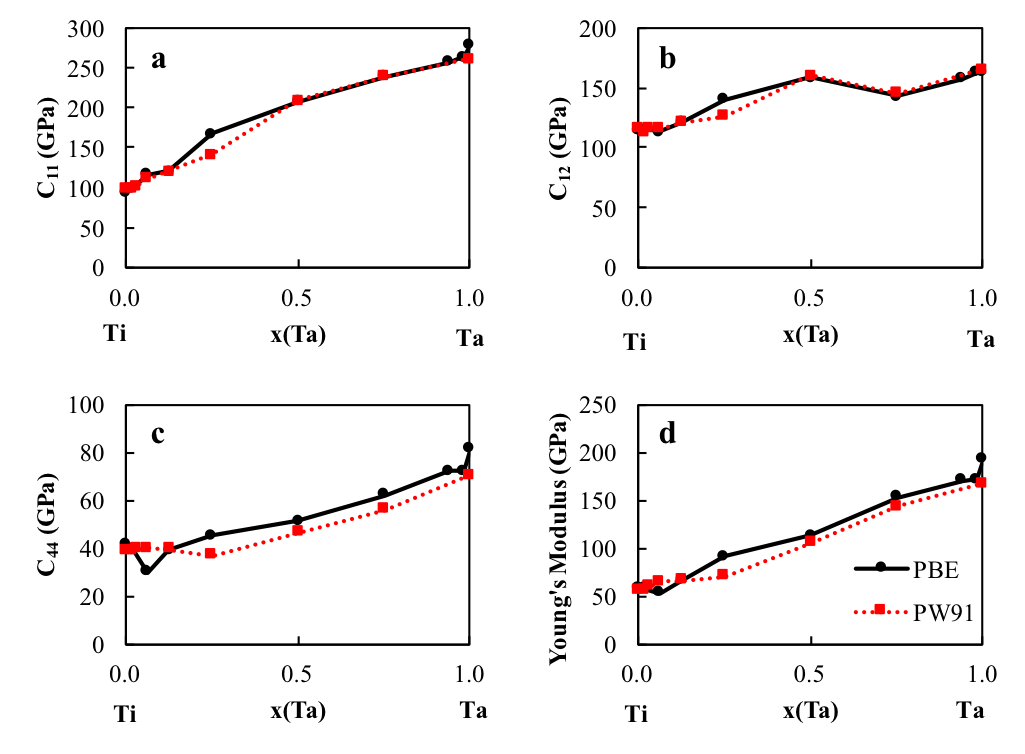
\includegraphics[width=\textwidth]{Chapter-5/Figures/PBEvsPW91.png}
	\caption{Elastic stiffness constants of the bcc Ti-Ta binary system calculated with the PW91 and PBE exchange correction functions, respectively.}
	\label{Ch5-figure:PBEvsPW91}
\end{figure}

\pagebreak
\begin{figure}[H]
	\centering
	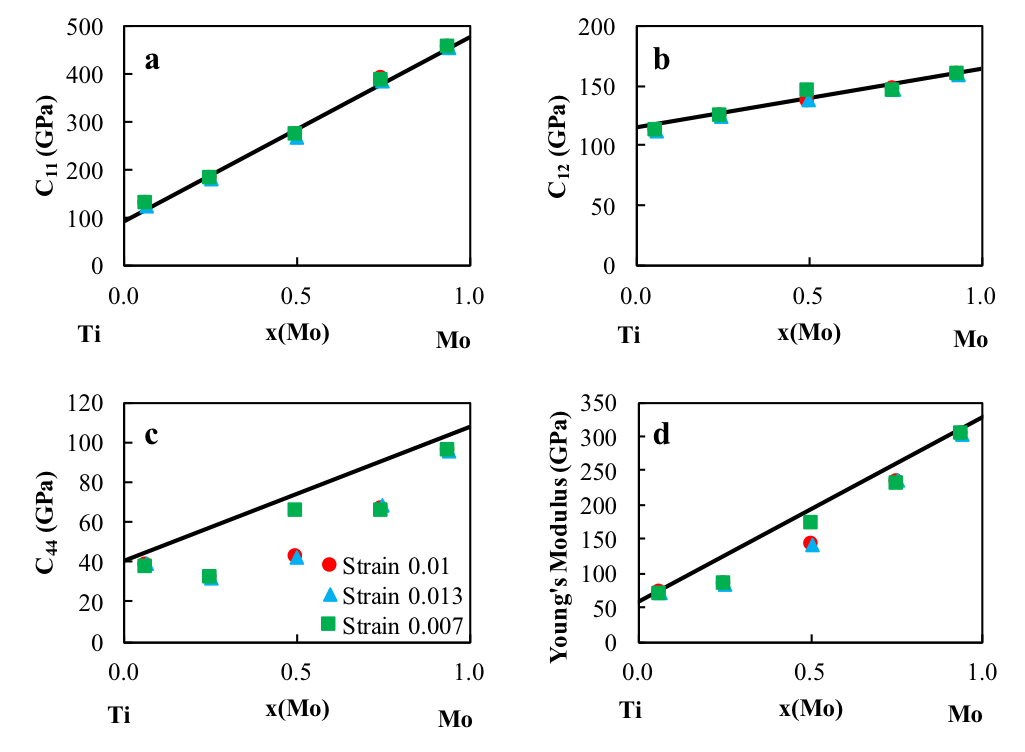
\includegraphics[width=\textwidth]{Chapter-5/Figures/Strain.png}
	\caption{Elastic stiffness constants for the bcc Ti-Mo binary system calculated with strains, $\pm$0.01, $\pm$0.013 and $\pm$0.07, respectively, showing comparable results.}
	\label{Ch5-figure:Strain}
\end{figure}

\pagebreak
\begin{figure}[H]
	\centering
	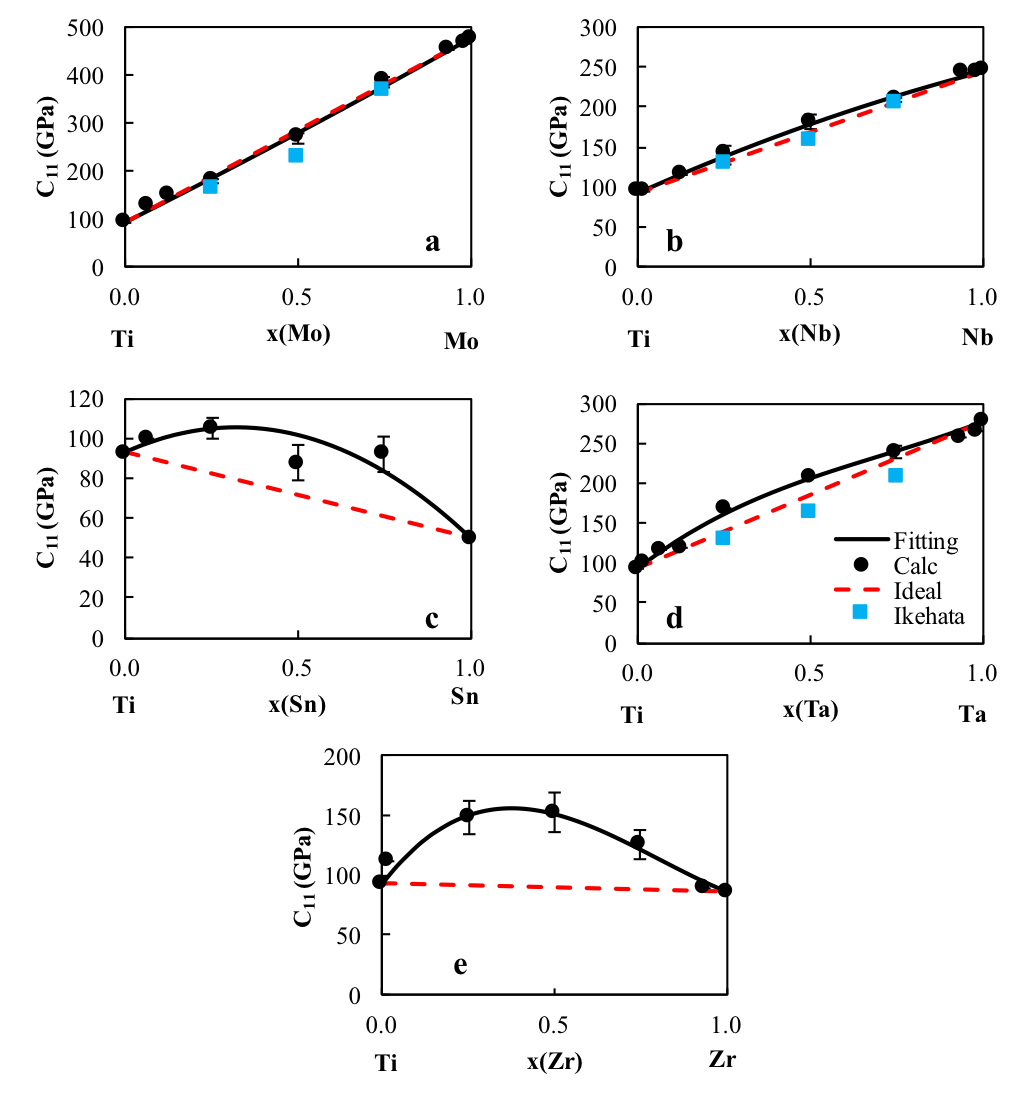
\includegraphics[width=\textwidth]{Chapter-5/Figures/tixc11.png}
	\caption{Calculated $\overline{C}_{11}$ values (circles) plotted with their errors as well as the linear combination of the pure element (red dashed line) and the present modeling (black dashed line) for five Ti-X binary systems (X = Mo, Nb, Ta, Sn, Zr). Ti-Mo, Ti-Nb, and Ti-Ta alloys are compared with previous calculations from Ikehata et al. \cite{Ikehata2004}.}
	\label{Ch5-figure:tixc11}
\end{figure}

\pagebreak
\begin{figure}[H]
	\centering
	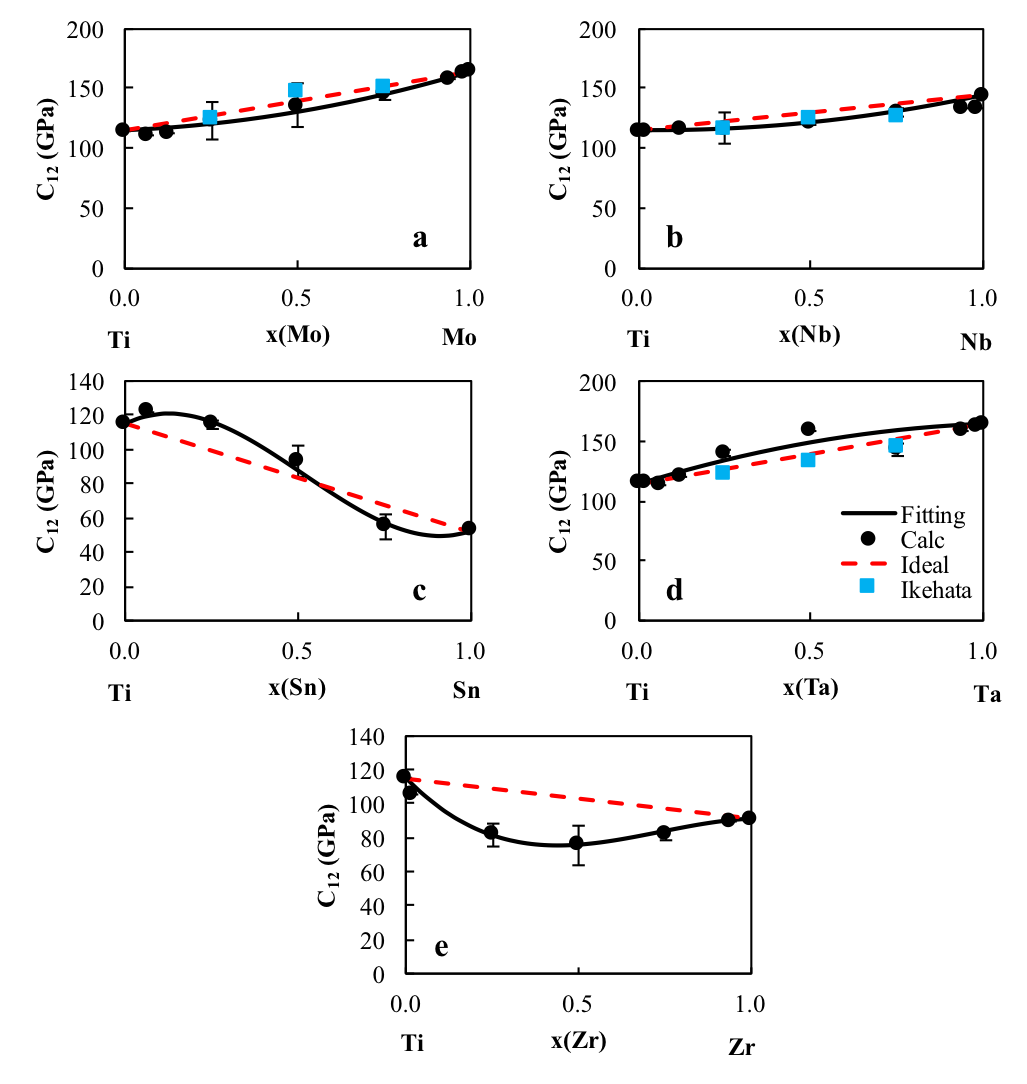
\includegraphics[width=\textwidth]{Chapter-5/Figures/tixc12.png}
	\caption{Calculated $\overline{C}_{12}$ values (circles) plotted with their errors as well as the linear combination of the pure element (red dashed line) and the present modeling (black dashed line) for five Ti-X binary systems (X = Mo, Nb, Ta, Sn, Zr). Ti-Mo, Ti-Nb, and Ti-Ta alloys are compared with previous calculations from Ikehata et al. \cite{Ikehata2004}.}
	\label{Ch5-figure:tixc12}
\end{figure}

\pagebreak
\begin{figure}[H]
	\centering
	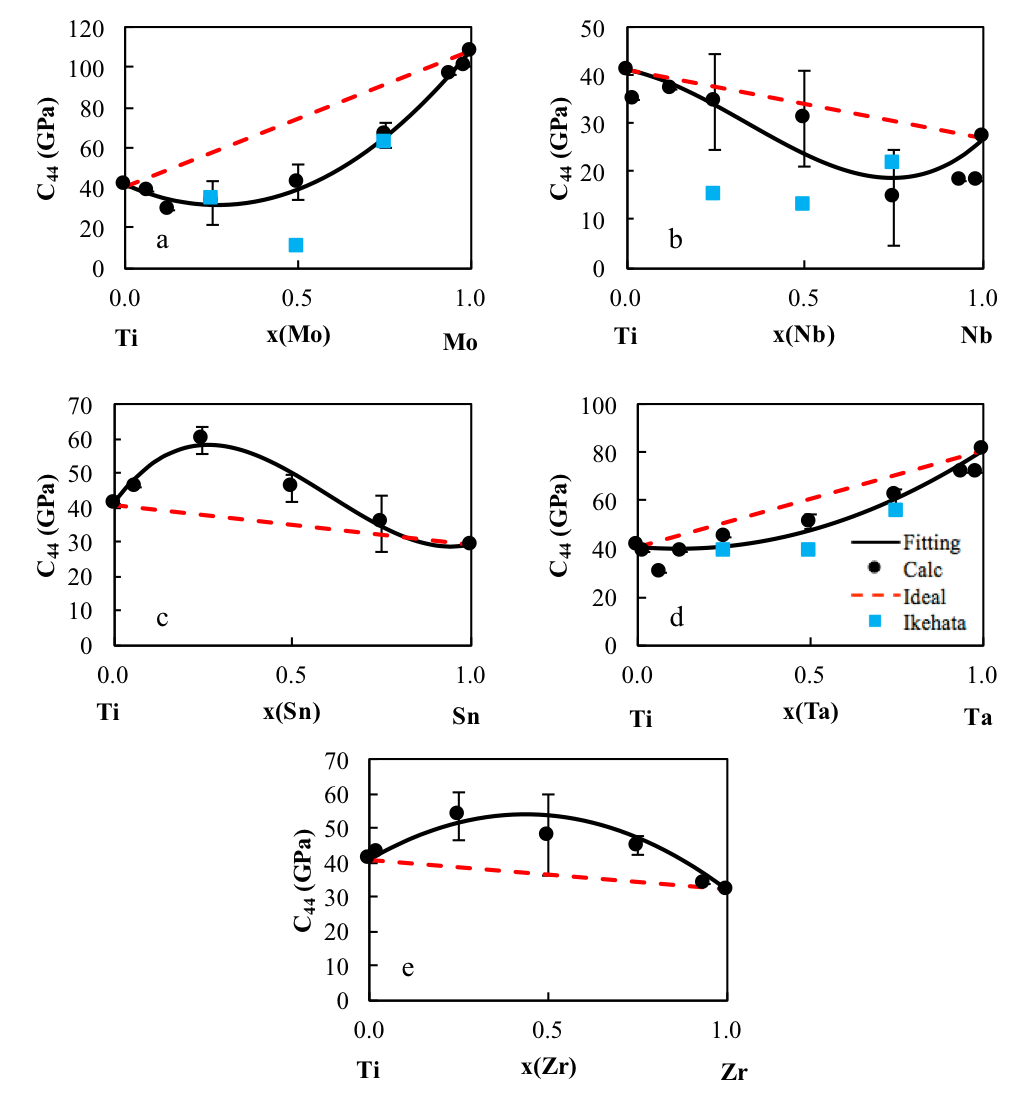
\includegraphics[width=\textwidth]{Chapter-5/Figures/tixc44.png}
	\caption{Calculated $\overline{C}_{44}$ values (circles) plotted with their errors as well as the linear combination of the pure element (red dashed line) and the present modeling (black dashed line) for five Ti-X binary systems (X = Mo, Nb, Ta, Sn, Zr). Ti-Mo, Ti-Nb, and Ti-Ta alloys are compared with previous calculations from Ikehata et al. \cite{Ikehata2004}.}
	\label{Ch5-figure:tixc44}
\end{figure}

\pagebreak
\begin{figure}[H]
	\centering
	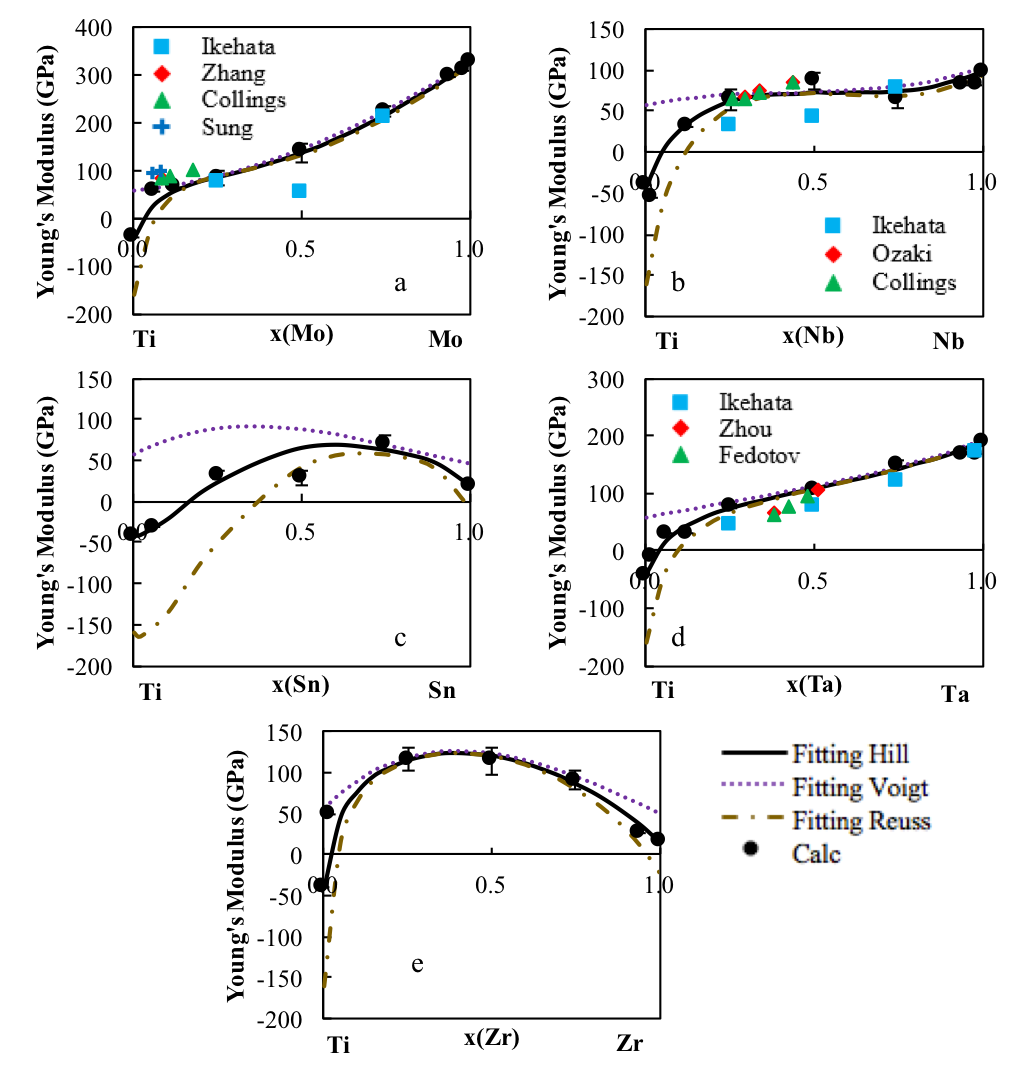
\includegraphics[width=\textwidth]{Chapter-5/Figures/tixyoungs.png}
	\caption{Young's modulus $E$ of the Ti-X binary systems. The present calculations are plotted as the filled circles with the error bars. The dotted purple line is the Voigt upper Young's modulus bound, the gold dot dashed line is the lower Reuss Young's modulus bound and the black line is the Hill Young's modulus average. The experimental values \cite{Ikehata2004,Zhang2015,Boyer1994,Sung2015,Ozaki2004,Fedotov1985,Zhou2009a,Zhou2004a,Friak2012,Wu2010a} are also included for comparison. }
	\label{Ch5-figure:tixyoungs}
\end{figure}

\pagebreak
\begin{figure}[H]
	\centering
	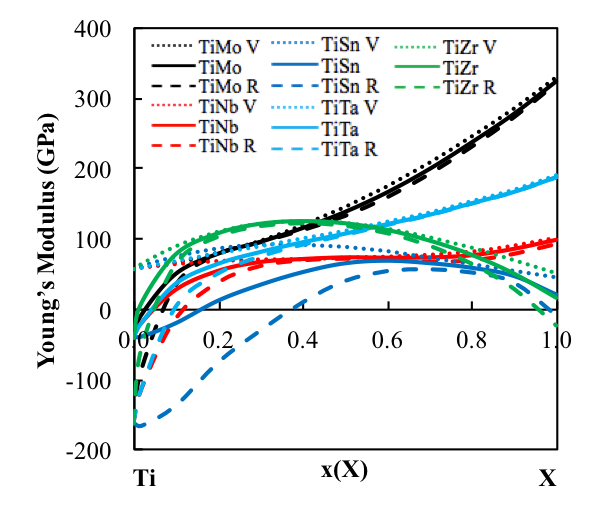
\includegraphics{Chapter-5/Figures/emap.png}
	\caption{Young's moduli mapped as a function of composition from bcc Ti to bcc X (X=Mo, Nb, Sn, Ta, Zr).}
	\label{Ch5-figure:tixmap}
\end{figure}

\pagebreak
\begin{figure}[H]
	\centering
	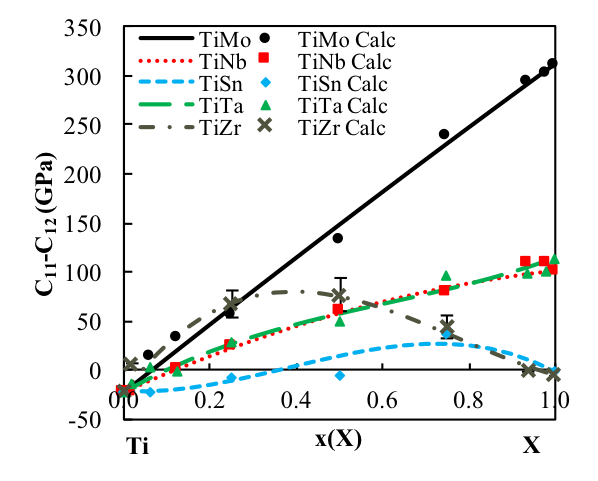
\includegraphics{Chapter-5/Figures/tixc11-c12.png}
	\caption{Calculated $\overline{C}_{11}$-$\overline{C}_{12}$ values (circles) plotted with the present modeling (solid lines) for five Ti-X binary systems (X = Mo, Nb, Ta, Sn, Zr). The $\overline{C}_{11}$-$\overline{C}_{12}$ shows the stability of the bcc phase. When the $\overline{C}_{11}$-$\overline{C}_{12}$ value is negative the bcc phase is not stable in the corresponding composition ranges.}
	\label{Ch5-figure:tixc11-c12}
\end{figure}

\pagebreak
\begin{figure}[H]
	\centering
	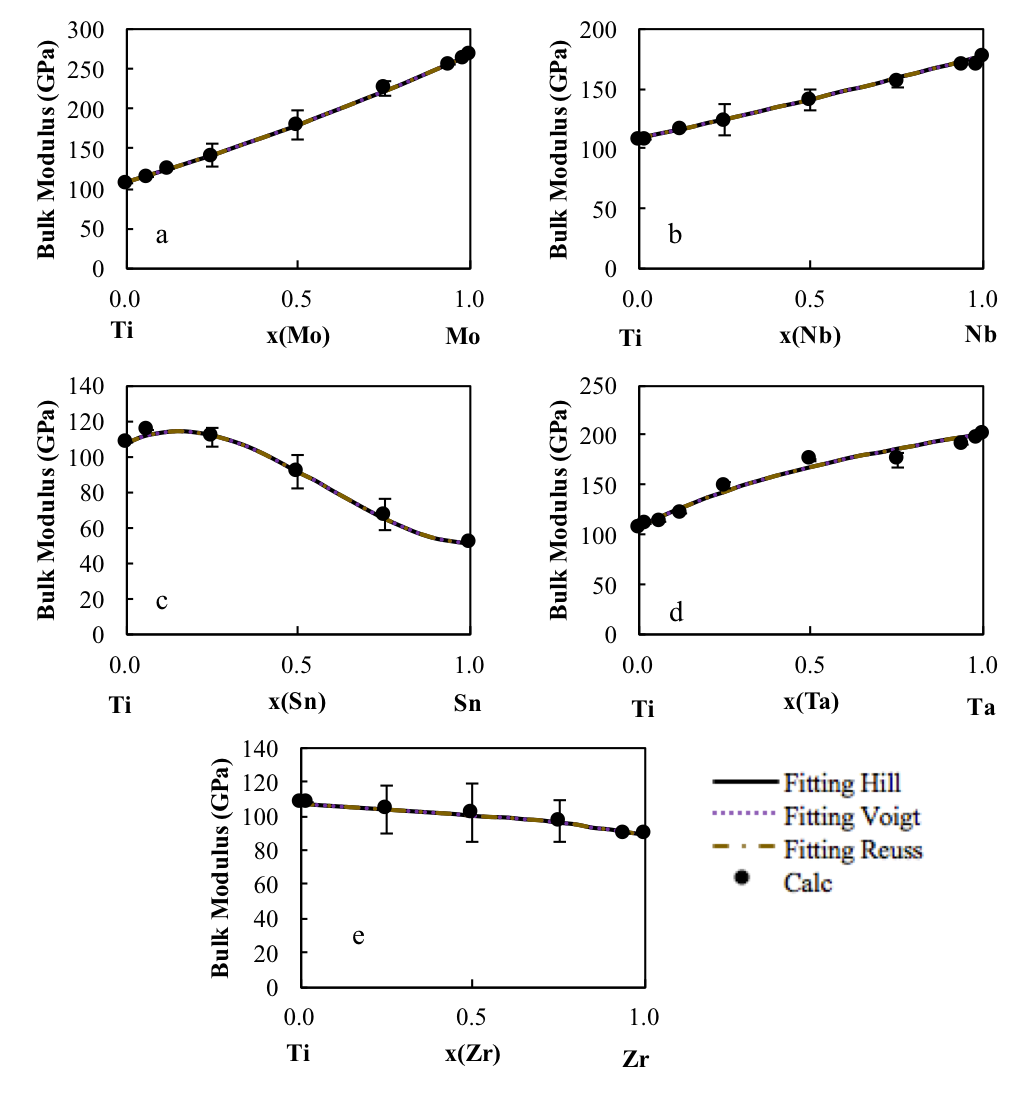
\includegraphics[width=\textwidth]{Chapter-5/Figures/tixbulk.png}
	\caption{Bulk moduli $B$ of the Ti-X binary systems. The present calculations are plotted as the filled circles with the error bars. The dotted purple line is the Voigt upper bulk modulus bound, the gold dot dashed line is the lower Reuss bulk modulus bound and the black line is the bulk modulus from the Hill approach.}
	\label{Ch5-figure:tixbulk}
\end{figure}

\pagebreak
\begin{figure}[H]
	\centering
	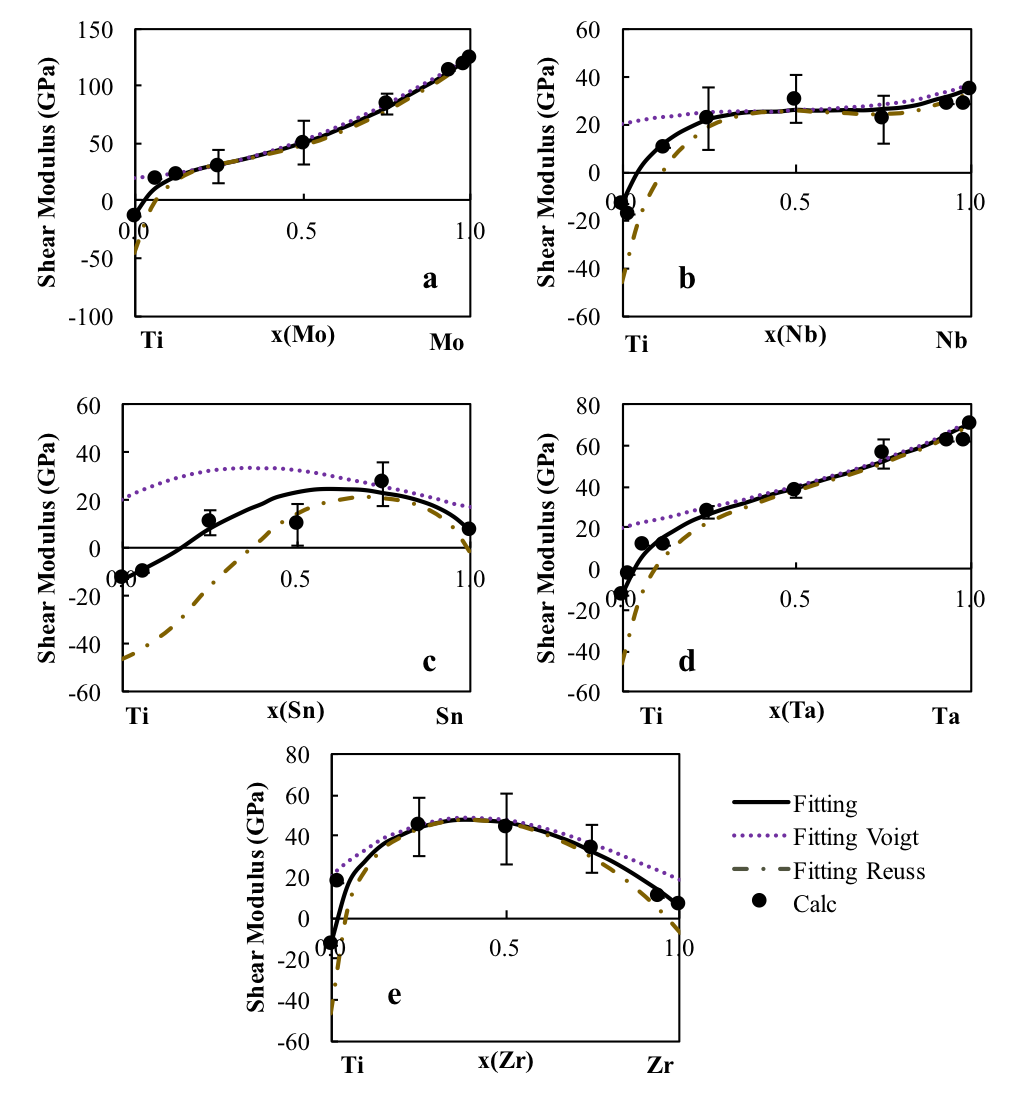
\includegraphics[width=\textwidth]{Chapter-5/Figures/tixshear.png}
	\caption{Shear moduli $G$ of the Ti-X binary systems. The present calculations are plotted as the filled circles with the error bars. The dotted purple line is the Voigt upper shear modulus bound, the gold dot dashed line is the lower Reuss shear modulus bound and the black line is the shear modulus from the Hill approach.}
	\label{Ch5-figure:tixshear}
\end{figure}

\pagebreak
\begin{figure}[H]
	\centering
	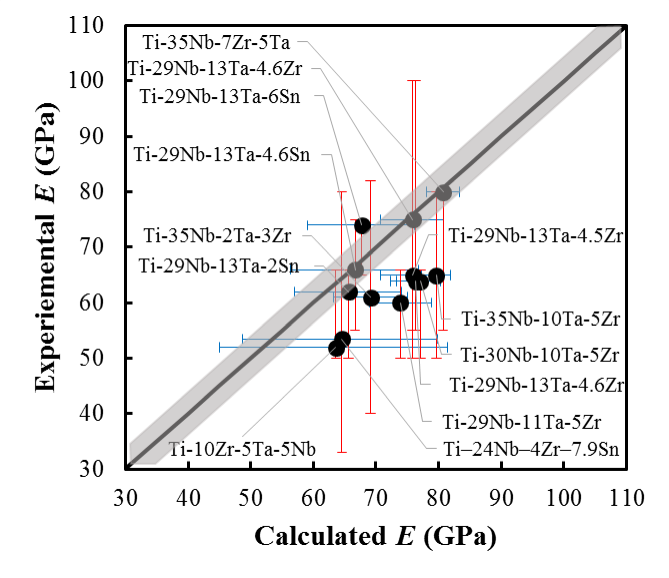
\includegraphics{Chapter-5/Figures/edatabase.png}
	\caption{Young's moduli values of multicomponent bcc Ti alloys measured experimentally plotted against the predicted Young's moduli from the pure elements and binary interaction parameters with the black diagonal line showing the exact correlation between the experimental and calculated values. Error in the experiments and the bounds from Reuss and Voigt approximations are plotted as the vertical and horizontal error bars, respectively. The variance in the first-principles calculations from Eq.\ref{eq: averagec11}-Eq.\ref{eq: averagec44} was averaged and plotted as the grey region. More information on the alloys is in Table \ref{Ch5-table:tixdatacomp} \cite{Tane2010a,Geetha2009,Mohammed2014}}
	\label{Ch5-figure:tixdatabase}
\end{figure}